
\newcommand{\blkb}{\cellcolor[rgb]{0,0,0}\textcolor{white} 0 }
\newcommand{\bwn}{\cellcolor[rgb]{.26,.22,0}\textcolor{white} 9 }
\newcommand{\ora}{\cellcolor[rgb]{.44,.31,.15}8 }
\newcommand{\red}{\cellcolor[rgb]{.6,.4,.35}A }
\newcommand{\lgr}{\cellcolor[rgb]{.58,.58,.58}F }
\newcommand{\yel}{\cellcolor[rgb]{.72,.78,.44}7 }

\newcommand{\redb}{\cellcolor[rgb]{.6,.4,.35} 1 }

\chapter{Graphics}
\label{cha:graphics}

Let's have some fun with graphics!
In this part of the book, we want to examine the MEGA65's graphics modes by walking through example code in machine language and BASIC to get to know the various options of the MEGA65 in the area of graphics. First of all, it is important to know that the MEGA65 supports three different basic graphics modes:

\begin{itemize}
	\item Bitmap graphics
	\item Graphics based on character sets
	\item Bitplanes
\end{itemize}


\section*{Bitmap Graphics}

In bitmap graphics every pixel of a graphic is stored separately. The way the pixels are hold in memory varies from system to system and in most cases depends on the performance of the hardware. If memory would be unlimited, the easiest way to remember a pixel is to save its RGB-values in three separate bytes. Example: 0xFFFFFF for white would result in three values to be stored: \$FF, \$FF and \$FF. To be honest, this is too simple and not really efficient. Let’s think about another way. Why not defining a color table (or color palette) and store the RGB values once and finally only reference the color by its index in the table? This will save us a lot of memory! Let's imagine we would create a colorful 8x8 bitmap to represent an "A" on the screen. Colourful means, we want it in some brownish colors. The color table for it may look like this:

\begin{center}
\begin{tabular}{|l|l|}
\hline
	Index & Color \\
\hline
	\blkb & Black \\
	\bwn & Brown \\
	\ora & Orange \\
	\red & Light Red \\
	\lgr & Light Grey \\
	\yel & Yellow \\
\hline
\end{tabular}
\end{center}

The color values, by the way, are exactly the same as the color values from the standard C64 color palette. Next we design the "A". Each pixel references a value from the color table above.


\begin{center}
\begin{tabular}{|m{6pt}|m{6pt}m{6pt}m{6pt}m{6pt}m{6pt}m{5pt}m{6pt}m{6pt}|}
\hline
	& 7 & 6 & 5 & 4 & 3 & 2 & 1 & 0 \\
\hline
	0 & \blkb & \blkb & \blkb & \blkb & \blkb & \blkb & \blkb & \blkb \\
	1 & \red & \lgr & \yel & \lgr & \red & \ora & \blkb & \blkb \\
	2 & \lgr & \lgr & \blkb & \blkb & \ora & \red & \blkb & \blkb \\
	3 & \yel & \yel & \blkb & \blkb & \ora & \red & \blkb & \blkb \\
	4 & \yel & \lgr & \lgr & \red & \red & \red & \blkb & \blkb \\
	5 & \lgr & \red & \blkb & \blkb & \ora & \red & \blkb & \blkb \\
	6 & \red & \red & \blkb & \blkb & \red & \red & \blkb & \blkb \\
	7 & \ora & \bwn & \blkb & \blkb & \ora & \red & \blkb & \blkb \\
\hline
\end{tabular}
\end{center}

But how much memory does this little graphic use?

If we create an one-dimensional array, we will get an array with 64 elements, because our graphic consists of 8x8 pixels = 64 color values that have to be saved. If we transfer that to the memory of the MEGA65, it means that we have 64 bytes to store in memory. However, full-screen graphics are made up of far more pixels. On the C64 and of course also on the MEGA65, 320x200 pixels are required to generate a graphic that fills the entire screen. If we transfer this to our array, we would have a total of 64,000 entries. Converted to the memory of the MEGA65, that is 64,000 bytes or nearly 64 kilobytes of data! If we now also consider that the good old C64 only had 64K of RAM available, we recognize the Drama! That's just too much data! We need strategies to reduce our bitmap data. On the C64 we had two types of bitmap graphics and both come with its own concepts to use as less memory as possible.

\begin{itemize}
	\item Hires
	\item Multicolor (MCM)
\end{itemize}


\subsection*{Hires}

First, a bitmap is divided into blocks of 8x8 pixels each. In order to achieve the full resolution of 320x200 pixels, 40 of such blocks next to each other builds up a line. If we now build up 25 lines, we arrive at a graphic that fills the complete screen.

\begin{adjustbox}{width=\textwidth,center}
\begin{footnotesize}
\begin{tabular}[h]{|C{10pt}|C{5pt}|C{5pt}|C{5pt}|C{5pt}|C{5pt}|C{5pt}|C{5pt}|C{5pt}|C{5pt}|C{5pt}|C{5pt}|C{5pt}|C{5pt}|C{5pt}|C{5pt}|C{5pt}|C{5pt}|C{5pt}|C{5pt}|C{5pt}|C{5pt}|C{5pt}|C{5pt}|C{5pt}|C{5pt}|C{5pt}|C{5pt}|C{5pt}|C{5pt}|C{5pt}|C{5pt}|C{5pt}|C{5pt}|C{5pt}|C{5pt}|C{5pt}|C{5pt}|C{5pt}|C{5pt}|C{5pt}|}
\hline
  &   &   &  &  &  &   &   &   &   & 1  & 1  & 1  & 1  & 1  & 1  & 1  & 1  & 1  & 1  & 2  & 2  & 2  & 2  & 2  & 2  & 2  & 2  & 2  & 2  & 3  & 3  & 3  & 3  & 3  & 3  & 3  & 3  & 3  & 3  & 4  \\
  & 1 & 2 & 3& 4& 5& 6 & 7 & 8 & 9 &  0 & 1  &  2 &  3 &  4 &  5 &  6 &  7 &  8 &  9 &  0 &  1 &  2 &  3 &  4 &  5 &  6 &  7 &  8 &  9 &  0 &  1 &  2 &  3 &  4 &  5 &  6 &  7 &  8 &  9 &  0 \\
\hline
   1 & & & & & & & & & & & & & & & & & & & & & & & & & & & & & & & & & & & & & & & & \\\hline
   2 & & & & & & & & & & & & & & & & & & & & & & & & & & & & & & & & & & & & & & & & \\\hline
   3 & & & & & & & & & & & & & & & & & & & & & & & & & & & & & & & & & & & & & & & & \\\hline
   4 & & & & & & & & & & & & & & & & & & & & & & & & & & & & & & & & & & & & & & & & \\\hline
   5 & & & & & & & & & & & & & & & & & & & & & & & & & & & & & & & & & & & & & & & & \\\hline
   6 & & & & & & & & & & & & & & & & & & & & & & & & & & & & & & & & & & & & & & & & \\\hline
   7 & & & & & & & & & & & & & & & & & & & & & & & & & & & & & & & & & & & & & & & & \\\hline
   8 & & & & & & & & & & & & & & & & & & & & & & & & & & & & & & & & & & & & & & & & \\\hline
   9 & & & & & & & & & & & & & & & & & & & & & & & & & & & & & & & & & & & & & & & & \\\hline
  10 & & & & & & & & & & & & & & & & & & & & & & & & & & & & & & & & & & & & & & & & \\\hline
  11 & & & & & & & & & & & & & & & & & & & & & & & & & & & & & & & & & & & & & & & & \\\hline
  12 & & & & & & & & & & & & & & & & & & & & & & & & & & & & & & & & & & & & & & & & \\\hline
  13 & & & & & & & & & & & & & & & & & & & & & & & & & & & & & & & & & & & & & & & & \\\hline
  14 & & & & & & & & & & & & & & & & & & & & & & & & & & & & & & & & & & & & & & & & \\\hline
  15 & & & & & & & & & & & & & & & & & & & & & & & & & & & & & & & & & & & & & & & & \\\hline
  16 & & & & & & & & & & & & & & & & & & & & & & & & & & & & & & & & & & & & & & & & \\\hline
  17 & & & & & & & & & & & & & & & & & & & & & & & & & & & & & & & & & & & & & & & & \\\hline
  18 & & & & & & & & & & & & & & & & & & & & & & & & & & & & & & & & & & & & & & & & \\\hline
  19 & & & & & & & & & & & & & & & & & & & & & & & & & & & & & & & & & & & & & & & & \\\hline
  20 & & & & & & & & & & & & & & & & & & & & & & & & & & & & & & & & & & & & & & & & \\\hline
  21 & & & & & & & & & & & & & & & & & & & & & & & & & & & & & & & & & & & & & & & & \\\hline
  22 & & & & & & & & & & & & & & & & & & & & & & & & & & & & & & & & & & & & & & & & \\\hline
  23 & & & & & & & & & & & & & & & & & & & & & & & & & & & & & & & & & & & & & & & & \\\hline
  24 & & & & & & & & & & & & & & & & & & & & & & & & & & & & & & & & & & & & & & & & \\\hline
  25 & & & & & & & & & & & & & & & & & & & & & & & & & & & & & & & & & & & & & & & & \\\hline
\end{tabular}
\end{footnotesize}
\end{adjustbox}

Splitting into blocks makes sense because this gives us the chance to reduce the data drastically. Each line of a 8x8 block are 8 bits, so why not forget the color indexes and just say each pixel set represents a "1" in the line and each pixel not set corresponds to "0".

\begin{center}
\begin{tabular}{|C{12pt}|C{12pt}C{12pt}C{12pt}C{12pt}C{12pt}C{12pt}C{12pt}C{12pt}|R{24pt}|R{24pt}|}
\hline
	& 7 & 6 & 5& 4& 3&  2& 1& 0 & dec & hex \\
\hline
0 & \blkb & \blkb & \blkb & \blkb & \blkb & \blkb & \blkb & \blkb &   0 & 00 \\
1 & \blkb & \redb & \redb & \redb & \redb & \blkb & \blkb & \blkb & 120 & 78 \\
2 & \redb & \redb & \blkb & \blkb & \redb & \redb & \blkb & \blkb & 204 & CC \\
3 & \redb & \redb & \blkb & \blkb & \redb & \redb & \blkb & \blkb & 204 & CC \\
4 & \redb & \redb & \redb & \redb & \redb & \redb & \blkb & \blkb & 252 & FC \\
5 & \redb & \redb & \blkb & \blkb & \redb & \redb & \blkb & \blkb & 204 & CC \\
6 & \redb & \redb & \blkb & \blkb & \redb & \redb & \blkb & \blkb & 204 & CC \\
7 & \redb & \redb & \blkb & \blkb & \redb & \redb & \blkb & \blkb & 204 & CC \\
\hline
\end{tabular}
\end{center}

As shown above now you can easily convert the bits of each line to its hex value and you finally get 8 bytes of data. This is the central idea in hires graphics and with this concept you save a lot of memory. Here in this example it's 8 bytes versus 64 bytes if you have to manage all the color references.
Let's count it up for a full screen picture: We have 40x25 blocks, that is 1000 blocks in total. Each block is 8 bytes or 1 kilobyte, so we'll result in "only" 10K for a full screen picture.\\

This is a brilliant solution, but now have a problem: We lost the colors!\\

If you look at the first figure, it was very colorful. But do we really need so many colors? This is the second important concept in hires bitmap graphics: Less colors means less memory. In fact hires mode limits you to \textbf{two colors} per 8x8 pixel block. This information is stored in the Screen-RAM, not in the Color-RAM as one might assume. And again the idea why is really clever: In Screen-RAM you can hold values between \$00 and \$FF whereas in the Color-RAM it makes only sense to store values between \$0 and \$0F to reference one specific color from the C64 color palette which consists of 16 colors (\$0-\$F). On the MEGA65 you can have even more colors and you are able to tweak the default colors, but this will be explained later.\\

Back to the Screen-RAM. Here you store \textbf{two colors} for each 8x8 block. If you split the byte into its Hi- and Low-Byte you have the chance to put a background and a foreground color into it! The value \$0a for example can be seen as \$0 and \$a. This way we'll get a black background and light red for the pixels in the block. In the end this means, a fullscreen hires bitmap will consume not 10 but 20 Kilobytes. 10K for the raw bitmap data as mentioned earlier and another 10K for the colors inside the Screen-RAM.\\

\subsection*{Programming simple Hires Bitmaps}

Let's code! But let's do it in BASIC first before we switch over to machine language. In order to bring bitmap graphics to the screen, we need to configure the VIC IV chip. There are several things VIC needs to know before it can find and read bitmap data. You have to do the following:

\begin{itemize}
	\item Make sure to have activated the VIC-registers you need (remember the MEGA65 offers different versions of the VIC-chip)
	\item Set the resolution
	\item Define a location for the bitmap data 
	\item And finally turn on bitmap mode
\end{itemize}

All these settings can be configured in different registers of your MEGA65. A reference of the existing registers for the graphics chip (which of course is the VIC) can be found in Appendix M. 

Your MEGA65 contains one graphics chip, the \textbf{VIC IV}, which builds on its two predecessors and adds new functions in the form of additional registers to it. These are the \textbf{VIC II} as it was used in the original Commodore 64 and the \textbf{VIC III aka "Bill"} as it was planned for the Commodore 65. 

It is important to understand that these different VIC-versions build on each other, think of it as modes you can turn on or off.
VIC III expands the existing registers of the VIC II while the VIC IV provides you with all existing registers of VIC II and VIC III, building on them by adding new functionality to previously unused registers. This means in Appendix M not only the registers for the VIC IV are important to know, but also those from VIC II and VIC III depending on which VIC-mode you have activated or not. Please keep this in mind.

\textbf{Make sure to have activated the VIC-registers you need} - what does this mean? Generally speaking you use the new register \$D02F hex or 53295 decimal to switch between VIC-modes or better to add or remove specific registers. In order to switch you use some kind of a "knocking-sequence" by poking two specific values one after the other: 

\begin{tabular}{|l|l|l|}
	\hline
	VIC & 1st hex/dec & 2nd hex/dec \\
	\hline
	II  & \$00/0 & \$00/0\\
	III & \$A5/165 & \$96/150\\
	IV  & \$47/71 & \$53/83\\	
	\hline
\end{tabular}

By the way, the two values you use to activate the VIC IV are in strings "G" and "S". These are the initials of the creator of the VIC IV: Dr. Paul Gardner-Stephen. Funny easteregg, isn't it? 

It is important to understand that, when you turn on your MEGA65, the computer will start in C64 mode and then looks for a C65-compatible ROM. If a C64 cartridge is detected or the MEGA-key is pressed the system stays in C64 mode. In this case, you only have the C64 registers available. If the system finds a C65 ROM, available registers will be activated. In case of the MEGA65 ROM this means, you can access all VIC-registers (II,III and IV). When you issue the GO64 command, the system will restrict you to the VIC II registers - but remember - by poking the knock-sequence as explained above you can add the registers again! This means it doesn't matter in which "mode" your are. All features are available from everywhere. The MEGA65 is a really flexible machine!


In this chapter we assume your are in a C65 mode using the standard MEGA65 ROM with BASIC65.


Next step is to \textbf{set the resolution}. According to the registers in Appendix M you can do this by using \$D031 hex, or 53297 decimal. This register is provided by VIC III. The C65 comes with a 80 column display, the C64 only had 40. In order to realize 80 columns, the graphics chip needs to be able to handle higher resolutions. When you turn on the computer you are in 80 column mode with 25 lines which is a 640x200 resolution. In order to show classic Bitmaps you need to reduce it down to 320x200 (which are the 40 columns and 25 lines as already shown in the table before). The C64 was not able to view 640x200, so no need for a register to control it on the VIC II. The C65 on the other hand is able to do both so you can use \$D031 to switch between them.  If you manipulate it by its bits you can control even more: resolution (databit 7, H640), C65 fast mode (databit 6, FAST) or turning off and on the new Bitplane-Mode as an alternative to classic bitmap- or char-based graphics (databit 4, BPM). There are also some registers which where planned, but never implemented. For example a H1280-Mode on databit 2 which should make the C65 able to scale up to 1280x200 or 1280x400. See Appendix M for the bloody details.

The next question is, how can we control specific bits in a register? If you turn on your computer and enter the following command

\begin{screenoutput}
PRINT PEEK($D031)
 224
\end{screenoutput}

you get back a decimal value like 224. The decimal value does not help, you need to convert the number into its binary representation. 

\begin{tabular}{|l|l|l|l|l|l|l|l|l|}
	\hline
	Bit 7 & Bit 6 & Bit 5 & Bit 4 & Bit 3 & Bit 2 & Bit 1 & Bit 0 & Decimal value \\
	H640 & FAST & ATTR & BPM & V400 & H1280 & MONO & INT & ~ \\
	\hline
    1 & 1 & 1 & 0 & 0 & 0 & 0 & 0 & 224 \\
    0 & 1 & 1 & 0 & 0 & 0 & 0 & 0 & 96 \\    
	\hline
\end{tabular}

The first line in the table shows the binary number for decimal 224, this should be the case when you turn on your MEGA65. Databit 7, H640-mode is activated as expected. In the second line you see the value you have to use when you want to reduce down to 320x200: databit 7 is set to 0, so H640-mode is turned off.

\begin{screenoutput}
POKE $D031,96
\end{screenoutput}

But wait, poking the value directly is not always the correct way. If you know exactly what you do or better which state each bit of the register should have, can you continue like this. Storing the value 96 means setting all the databits. This is not always what we want. In some cases we might manipulate one specific bit, for instance databit 7 for the resolution while keeping the other bits in their existing state. You can achieve this with logical operations using the AND or OR operator.

\begin{tabular}{ ccc }   
	~ & ~ & ~ \\  
	% first table (AND)
	\begin{tabular}{ |c|c| } 
		\hline
		Operation & Result \\
		\hline
		0 AND 0 & 0  \\
		1 AND 0 & 0  \\
		0 AND 1 & 0  \\
		1 AND 1 & 1  \\						
		\hline
	\end{tabular} &  
    % some space between the two tables
	\begin{tabular}{c}
	    \hspace{1cm} \\
	\end{tabular}
	% second table (OR)
	\begin{tabular}{ |c|c| } 
   	    \hline
        Operation & Result \\
		\hline
		0 OR 0 & 0  \\
		1 OR 0 & 1  \\
		0 OR 1 & 1  \\
		1 OR 1 & 1  \\						
		\hline	
	\end{tabular} \\
\end{tabular}

The table above is important because it shows, how the bits will be modified if you put an operator on it. If you think about the idea of logical operations, you will see that you can use AND to set one specific bit and OR to get the exact opposite result. To be honest, this method can not only be used to set a single bit, but also to change any number of bits but to keep things simple we modify only one. Back to the "bad" poke of 96 what we've seen above, it could be better written like this:

\begin{screenoutput}
POKE $D031, PEEK($D031) AND 127 :REM SET BIT 7
POKE $D031, PEEK($D031) OR 128  :REM UNSET BIT 7
\end{screenoutput}

So that you understand this operations, again you need to convert the decimal numbers into its binary format. Next we apply the AND / OR operations bit by bit according to the rules in the table above to it. 
\begin{tabular}{ ccc }   
	~ & ~ & ~ \\  
	\begin{tabular}{|l|l|l|}
		\hline
		~ &  Binary & Decimal\\
		\hline
		~ & 11100000 & 224\\
		AND & 01111111 & 127\\
		\hline
		Result & 01100000 & 96\\
		\hline
	\end{tabular} &
	% some space between the two tables
	\begin{tabular}{c}
		\hspace{1cm} \\
	\end{tabular}
	\begin{tabular}{|l|l|l|}
		\hline
		~ &  Binary & Decimal\\
		\hline
		~ & 01100000 & 96\\
		OR & 10000000 & 128\\
		\hline
		Result & 11100000 & 224\\
		\hline
	\end{tabular} \\
\end{tabular}

You can test this, by the way, with some simple PRINT commands:

\begin{screenoutput}
PRINT 224 AND 127
  96

PRINT 96 OR 128
  224
\end{screenoutput}

Armed with this knowledge, we can now start configuring the VIC to show bitmap graphics. For this we have to fine-tune a number of registers but before we can start with that, we need to understand a bit more about the graphics chip, how it is organized and most importantly how it accesses the memory.

\subsection*{VIC IV organization and memory access basics}

In contrast to the cpu of your MEGA65, which can address 64KB at once, the VIC unfortunately is not able to this. It can only see 16KB, so you have to define exactly which 16KB it is allowed to see. To achieve this, the 64KB of Bank 0 (this is the memory bank where VIC is living and getting ins data) is divided into blocks of 16KB each. These 16KB blocks are called "video banks" or "VIC banks".

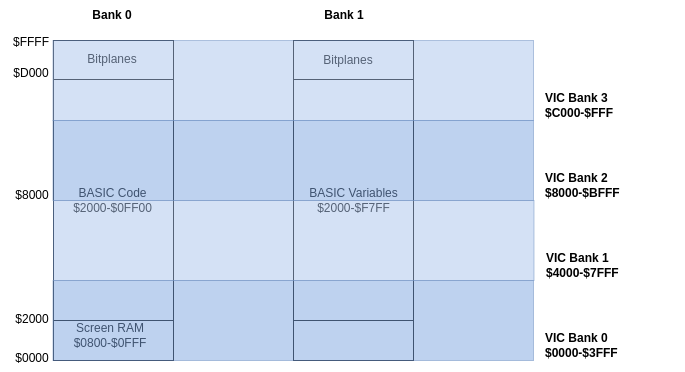
\includegraphics[width=\linewidth]{images/graphics/vic-banks.png}

Independent of the VIC, the memory management of the Commodore 65 or MEGA65 is somewhat more complex than that of the previous model. This is because there is more memory available in the machine: For the Commodore 65 128KB where planned and the MEGA65 comes with 384KB which can be scaled up to max 1 MB. As already mentioned, the processor is not able to address the whole range of memory. Only 64KB can be seen. For this reason the memory is divided into blocks, 64KB each, and these blocks are called "banks". The system can have up to 16 banks and certain banks also have certain tasks. Bank 0 for example is called the system bank, coming from BASIC65, this is the bank where VIC lives. The same applies to the screen RAM, which occupies the memory range \$0800-\$2000 after switching the computer on. This is also in bank 0. Banks 0 and 1 are RAM, which means you can read and write to them, while banks 2 and 3 are ROM and not so easy to override. By the way, the BASIC65 implementation itself is stored in the banks listed last. If you want to know more about memory management in general please have a look at Appendix F (System Memory Map). In BASIC - sorry to say - the situation is getting even more complex. Right after turning on the computer you are in Bank 128 which is a special bank with a special memory configuration. You can use the command BANK to switch between banks. A problem here is, that you can easily lose track of what is in which bank or in which bank you are currently working. It's actually a bit easier when working in machine language. For more information about the BANK-command and banks in special, please look into Appendix B (BASIC65 Command Reference). Please keep in mind that you need to know about banks, before you can safely use PEEK, POKE or SYS. Otherwise you may wonder why your program does not behave as expected. We will come back to this later. Back to graphics. 

Let's begin to write a simple BASIC programm to show hires bitmap graphics. If you followed this chapter carefully up to this point, you should have no trouble understanding the following lines of code:

\begin{screenoutput}
10 POKE $D020,0 : POKE $D021,0          :REM MAKE SCREEN BLACK
20 POKE $D031, PEEK($D031) AND 127      :REM SET RESOLUTION
30 POKE $DD02, 3                        :REM MAKE VIRTUAL CIA-2 READ- AND WRITEABLE 
40 POKE $$DD00, PEEK($DD00) AND 252 OR 2:REM SELECT VIDEO BANK 1
\end{screenoutput}

As you have seen in the illustration on the page before, the VIC chip divides the memory into 4 video banks of 16KB each. It is important to understand that you do not use a register of the VIC to define the video bank inside the (memory-)bank 0, instead you use the data bits 0 and 1 of \$DD00 or 56576 decimal. This used to be a register of the CIA-2 chip on the Commodore 64 but in your MEGA65 it is implemented as a virtual register. The "preparation" needed to set the video bank happens in line 30 while in the following line the video bank itself is set. By the way, when you convert the decimal value 3 (line 30) into its binary format, it is 00000011 and proves: the data bits 0 and 1 are set to 1, so reading and writing is activated.

\begin{tabular}{|c|c|l|l|}
	\hline
	Bits & VIC bank & Memory Area & BASIC \\
	\hline
	 \textbf{00} & 3 & \$C000-\$FFFF & ... AND 252 OR 0 :REM AND 11111100 OR 000000\textbf{00} \\
	 \textbf{01} & 2 & \$8000-\$BFFF & ... AND 252 OR 1 :REM AND 11111100 OR 000000\textbf{01} \\
	 \textbf{10} & 1 & \$4000-\$7FFF & ... AND 252 OR 2 :REM AND 11111100 OR 000000\textbf{10} \\
	 \textbf{11} & 0 & \$C000-\$3FFF & ... AND 252 OR 3 :REM AND 11111100 OR 000000\textbf{11} \\
	\hline
\end{tabular}

The table shows which bits must be set to select a video bank. 